\section{Methodology}
\label{sec:methodology}
% Focus on what you add to the existing method. Explain what you will do and why (and how). Do not forget to characterize your research design. There should be an evaluation plan in this section. (For DS students, this normally means using manually labelled or ground truth data.)

\subsection{Signal analysis pipeline}

The overall objective of this work is to increase the efficiency of the \texttt{Peregrine} data analysis pipeline. The work will begin with reproducing the results from papers \cite{bhardwaj2023peregrine} and \cite{alvey2023things}, as this will form the benchmark to which the eventual results will be compared to.

The workflow for the simulation-based inference technique for the analysis of the gravitational wave signals as implemented in \texttt{peregrine} \cite{bhardwaj2023peregrine} is shown in Figure \ref{fig:peregrine_pipeline}. The process starts by setting the 15 parameters of the `target observation' and then generating the example waveform to be analysed. This is done so there are `ground-truth' parameter values that you can compare your final posterior probability density distributions with to validate the overall method. If we use a true experimentally measured signal, then we can not know for certain what the `ground-truth' values of the parameters are. Given the accuracy that we can forward model the GW signals with, once the method is validated with the simulated waveforms, it is expected to work equally well with true experimental measurements.

\begin{figure}[htb]
    \centering
    \begin{tikzpicture}[node distance=2cm]
        \node (sampling) [sample] {\textbf{Sample} parameters $\boldsymbol{\theta}_{GW}$ from prior $p(\boldsymbol{\theta}_{GW})$};
        \node (fsimulator) [simulator, below of=sampling] {\textbf{Simulate} data $\boldsymbol{x}(\theta_{GW}) = h(\theta_{GW}) + n_{IFO}$};
        \node (network) [network, below of=fsimulator, yshift=-0.25cm] {\textbf{Train} CNN to estimate likelihood-to-evidence ratios $r(\boldsymbol{x};\theta_k) = p(\theta_k|\boldsymbol{x})/p(\theta_k)$ for all parameters $k$};
        \node (inference) [inference, below of=network] {Bayesian \textbf{Inference}};
        \node (prior) [pinput, left of=inference, xshift=-1cm] {Prior sample from $p(\theta)$};
        \node (target) [tinput, right of=inference, xshift=1cm] {Target Observation $\boldsymbol{x}_0$};
        \node (ratios) [output, below of=inference, xshift=-1.5cm] {Ratios $r(\boldsymbol{x}_0;\theta)$};
        \node (posterior) [output, below of=inference, xshift=1.5cm] {Posteriors $p(\theta|\boldsymbol{x}_0)$};
        \draw [arrow] (sampling) -- node[anchor=west] {$\boldsymbol{\theta}_{GW}$} (fsimulator);
        \draw [arrow] (fsimulator) -- node[anchor=west] {$\boldsymbol{\theta}_{GW},\boldsymbol{x}$} (network);
        \draw [arrow] (network) -- (inference);
        \draw [arrow] (prior) -- (inference);
        \draw [arrow] (target) -- (inference);
        \draw [arrow] (inference) -- (posterior);
        \draw [arrow] (inference) -- (ratios);
        \draw [arrow] (ratios) -- +(-3,0) |- node[anchor=west, yshift=-2cm, text width=2cm]{Using $r(\boldsymbol{x}_0;\theta)$ update prior $p(\boldsymbol{\theta}_{GW})$ and repeat until converged} (sampling);
    \end{tikzpicture}
    \caption{High-level overview of the simulation-based inference method used for this work.}
    \label{fig:peregrine_pipeline}
\end{figure}

\subsection{Data simulation}

The GW waveform data used to train the neural network is generated using the Bilby code \cite{Ashton_Bilby_2019} from input parameters that have been randomly sampled from prior distributions. We will investigate whether some more active learning can be introduced to increase the efficiency of the sampling process. For instance, some parameters such as the chirp mass\footnote{The chirp mass is a combination of the two object masses in the binary system, and is a key factor in the gravitational wave frequency as the two objects spiral inwards toward each other.\\$\mathcal{M} = \frac{(m_1 \cdot m_2)^{3/5}}{(m_1 + m_2)^{1/5}}$} may be inferred early on with relatively high confidence, but currently in subsequent simulation rounds continues to be sampled from a uniform distribution within $\pm5\sigma$ \cite{Miller_TMNRE_2021}. By being more selective in the sampling of parameters that are known with relatively high confidence, we can focus the simulation budget more on the parameters we know with less confidence. To do this in a systematic way, a complete survey of how influential each parameter is on the different segments of the GW signal will be carried-out first.

\subsection{Optimisation of network architecture}

The architecture of the network currently implemented in \texttt{peregrine} is the U-Net architecture \cite{Ronneberger_UNet_2015}. Given the advances in machine learning and CNN architectures since 2015, it is believed that this network can be improved upon. The optimisation of this network architecture will be the main focus of this thesis. 

Investigative studies will be performed to find the best network architectures most suitable for the data format. In this specific case, the data consists of 1D signals in both time and frequency domains, collected from three separate detectors that have captured the event simultaneously. An example of the signal in the time domain is shown in Figure \ref{fig:obs_time_domain}. In total, there are 8192 channels corresponding to 4\,s of collection time at a sampling frequency of 2048\,Hz. Through the Fourier transform, the time signal can be decomposed into its constituent frequency components. Both the time and frequency domains are fed into the network, since they have different information about the GW encoded. An example of the signal in the frequency domain is shown in Figure \ref{fig:obs_freq_domain}.

The chosen network architecture also needs to be capable of segmenting the signal into three components, representing the different stages of the merger event -- inspiral, merger and ringdown \cite{Pan_GW_2014}. Each of the parameters in $\boldsymbol{\theta}_{GW}$ are impacted differently in the different phases \cite{bhardwaj2023peregrine}.

\begin{figure}
  \centering
  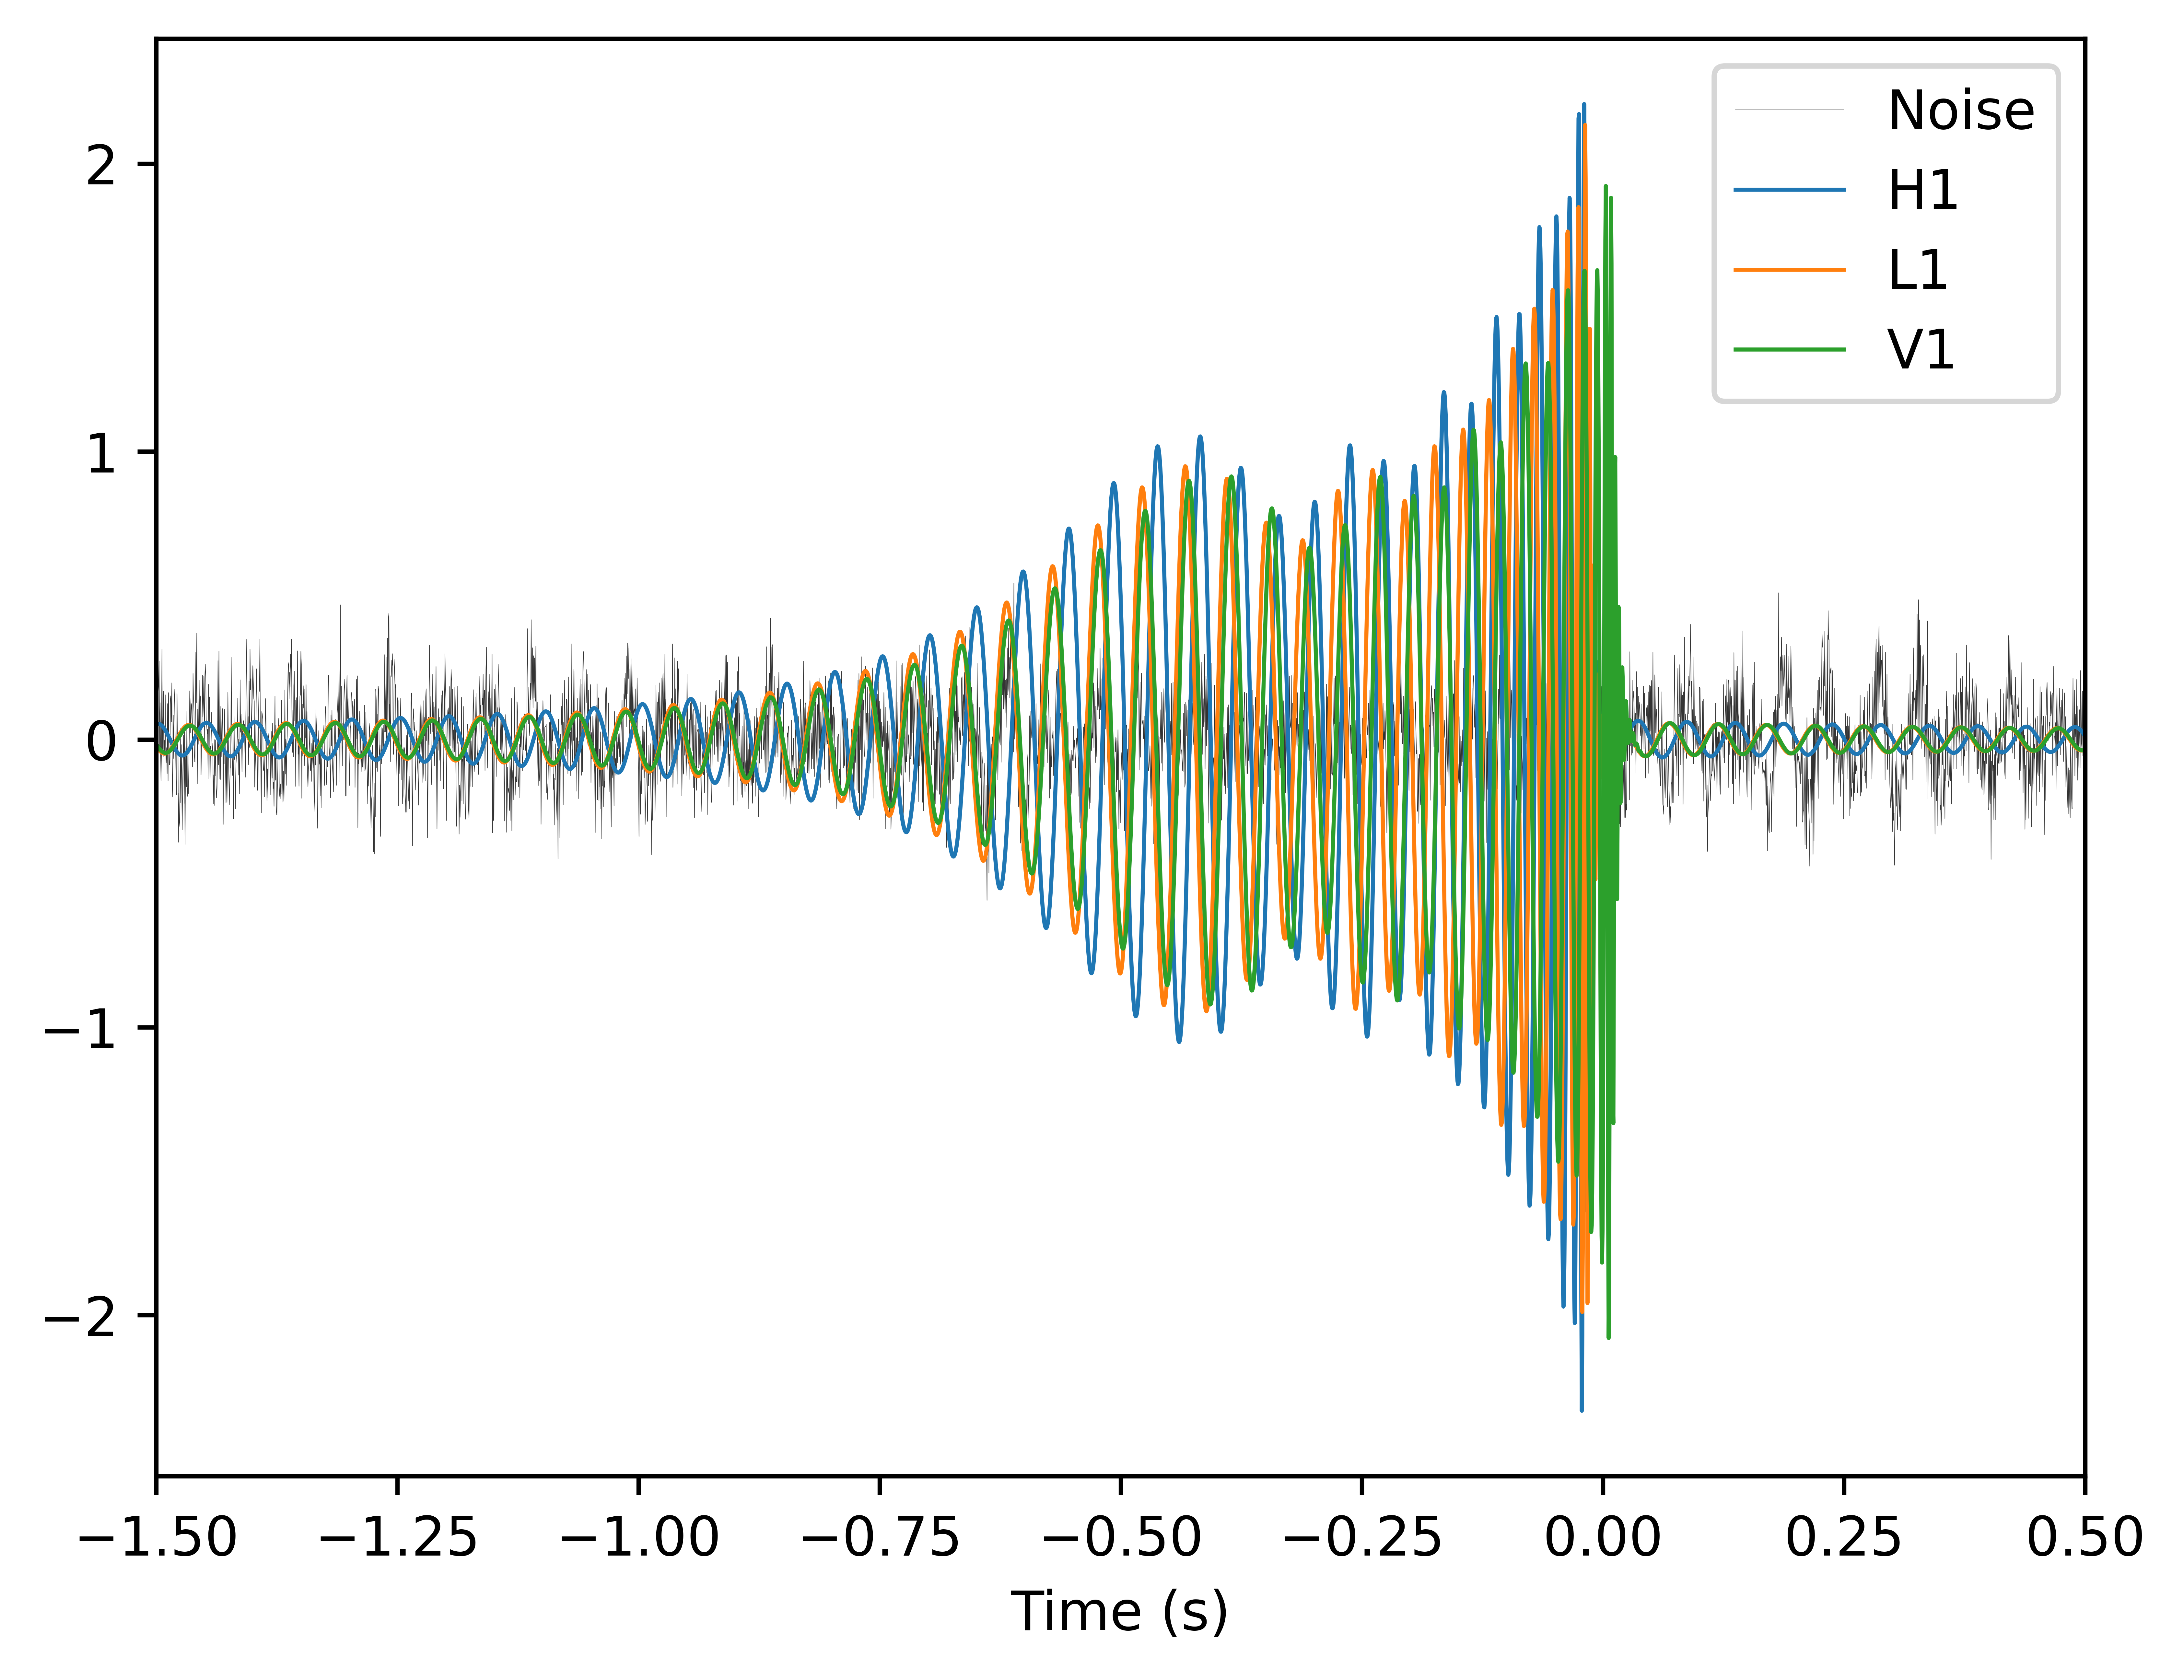
\includegraphics[width=1\linewidth]{media/images/obs_time_domain.png}
  \caption{Example of generated gravitational wave signal in the time domain. The noise and signal are shown separately in the figure, but are added together for training. The two black holes merge at the moment t=0s. }
  \label{fig:obs_time_domain}
\end{figure}

\begin{figure}
  \centering
  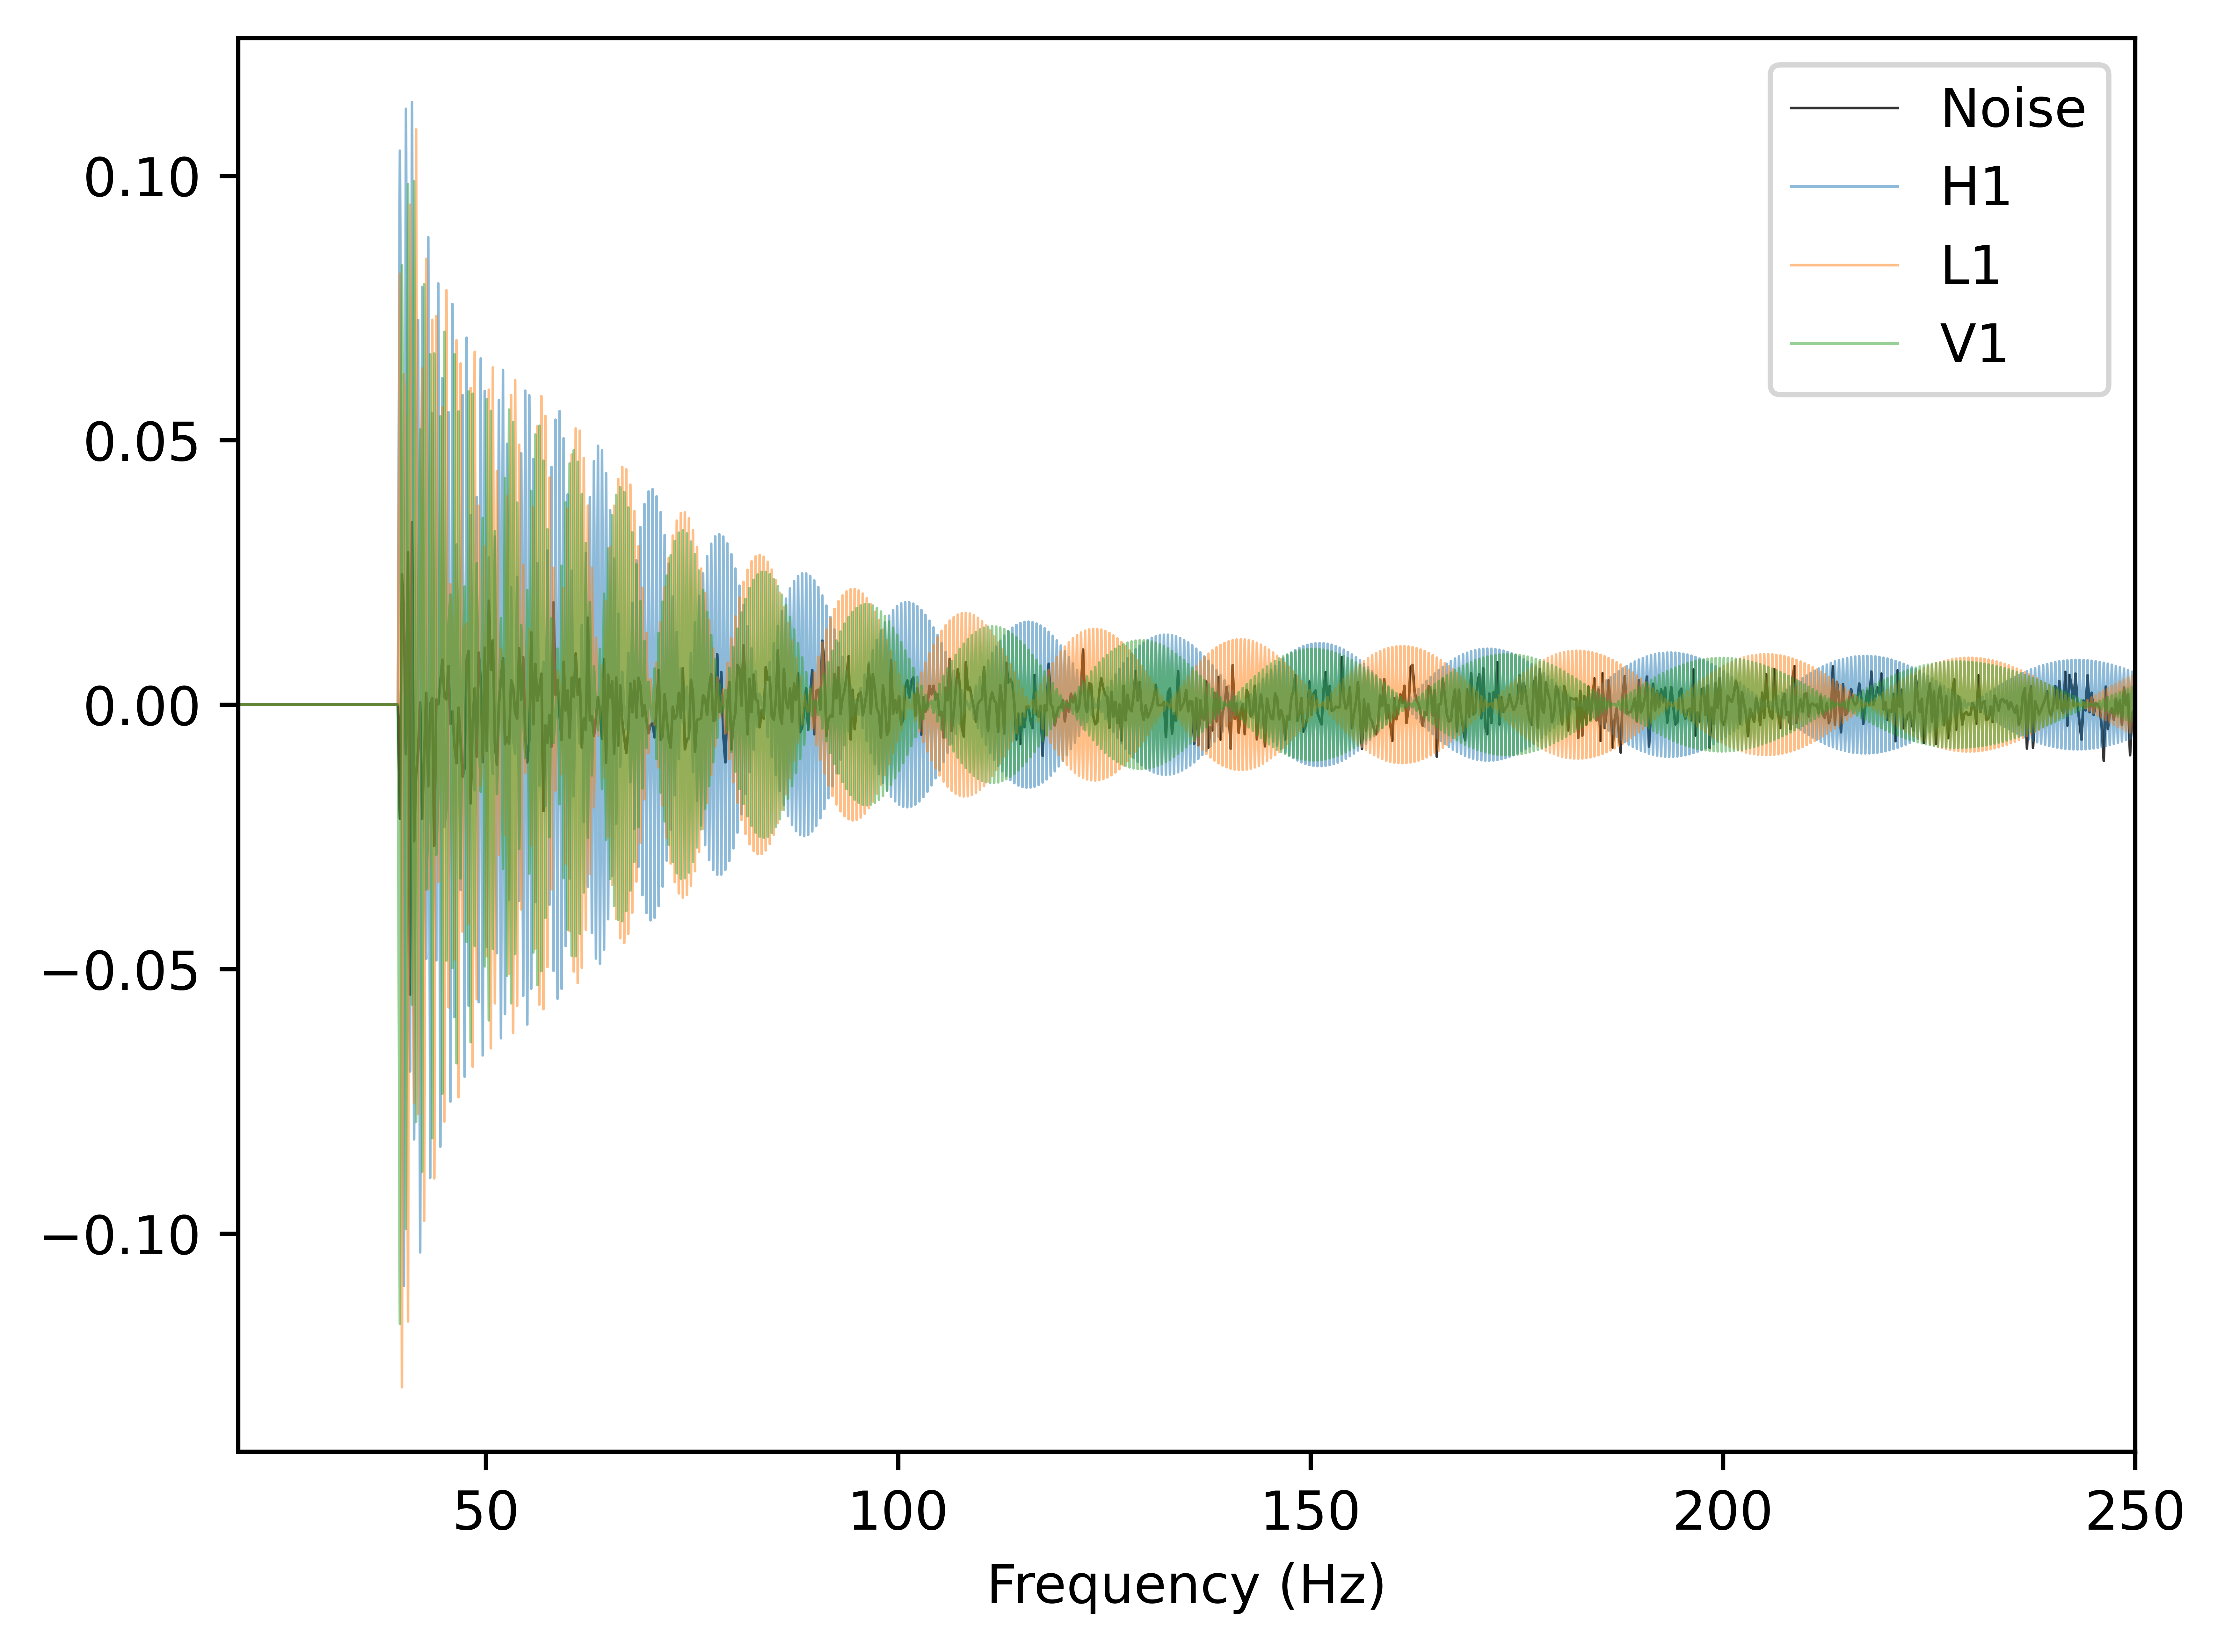
\includegraphics[width=1\linewidth]{media/images/obs_frequency_domain.png}
  \caption{Example of generated gravitational wave signal in the frequency domain. The noise and signal are shown separately in the figure, but are added together for training.}
  \label{fig:obs_freq_domain}
\end{figure}

\subsection{Evaluation}

The changes to the \texttt{peregrine} analysis pipeline will be fully benchmarked against the original \texttt{peregrine}, both in terms of accuracy of final result and required runtime. The results of the original \texttt{peregrine} have themselves been benchmarked against established likelihood-based methods \cite{Speagle_2020}, and found to be in good agreement. Therefore, in this work we think it is sufficient to compare only with the original \texttt{peregrine}. To demonstrate the applicability of the method to real gravitational wave measurements, if time permits, we will also test the approach using real experimental data.

